\documentclass{article}
\usepackage{amsmath}
\usepackage{enumitem}
\usepackage{graphicx}  % Add this to your preamble at the top of the document
\begin{document}

\section*{HW1 Computational Neurosceince}
\subsection*{Sepehr Saeedpour}

\section{Static action choice and reward}

\subsection*{(a)}
The sum of probabilities is:
\begin{align}
p(c=1) + p(c=2) = \frac{\exp(\beta m_1)}{\exp(\beta m_1) + \exp(\beta m_2)} + \frac{\exp(\beta m_2)}{\exp(\beta m_1) + \exp(\beta m_2)}\\
= \frac{\exp(\beta m_1) + \exp(\beta m_2)}{\exp(\beta m_1) + \exp(\beta m_2)} = 1.
\end{align}
Thus, \(\sum_{c=1}^2 p(c) = 1\).

\subsection*{(b)}
Divide numerator and denominator of \(p(c=1)\) by \(\exp(\beta m_1)\):
\begin{align}
p(c=1) = \frac{1}{1 + \exp(\beta(m_2 - m_1))}.
\end{align}


As $(m_2 - m_1) \to +\infty$, $p(c=1) \to 0$. As $(m_2 - m_1) \to -\infty$, $p(c=1) \to 1$.

\subsection*{(c) \& (d)}


\begin{figure}[h]
    \centering
    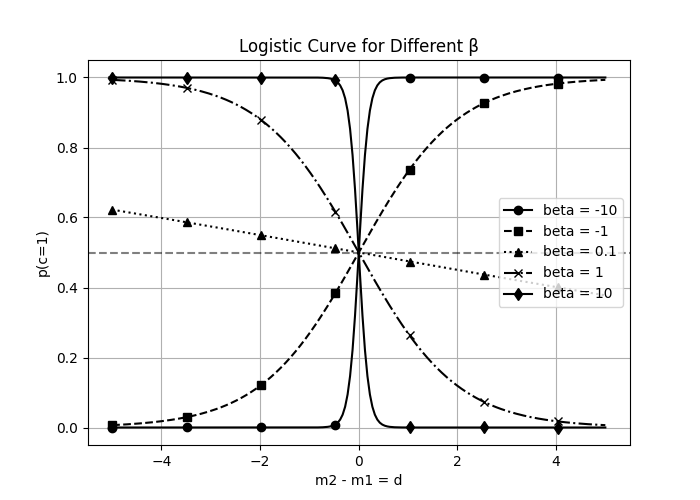
\includegraphics[width=0.7\textwidth]{logistic_curve.png}
    \caption{Probability of choosing blue flower as a function of reward difference $d = m_2 - m_1$.}
    \label{fig:softmax-choice}
\end{figure}
For \(d = m_2 - m_1\) and \(\beta = 1\), \(p(c=1)\) forms a sigmoid curve centered at \(d = 0\).

\begin{itemize}
    \item \textbf{Large \(d > 0\):} \(p(c=1) \to 0\) (bee avoids blue flowers).
    \item \textbf{Large \(d < 0\):} \(p(c=1) \to 1\) (bee strongly prefers blue flowers).
    \item \textbf{\(d \approx 0\):} \(p(c=1) \approx 0.5\) (balanced exploration).
\end{itemize}
The bee exploits clear reward differences but explores when rewards are similar.

\textbf{Parameter \(\beta\) (see Fig 1): }
\begin{itemize}
    \item \(\beta \to \infty\): Choices become deterministic (pure exploitation).
    \item \(\beta \to 0\): Uniform probabilities (pure exploration).
    \item \(\beta < 0\): Inverts preferences (illogical; standard \(\beta > 0\)).
\end{itemize}
\textbf{Tradeoff:} High \(\beta\) emphasizes exploitation; low \(\beta\) promotes exploration.

\subsection*{(e)}
For \(N\) flowers, generalize the softmax policy:
\begin{align}
p(c=i) &= \frac{\exp(\beta m_i)}{\sum_{j=1}^N \exp(\beta m_j)}.
\end{align}

Adjust \(\beta\) to balance exploration (low \(\beta\)) and exploitation (high \(\beta\)). 
Optimal learning often requires starting with lower $\beta$ values to encourage exploration and gradually increasing it to focus on exploitation

\subsection*{(f)}'




When the rewards $r_i(t)$ of the $N$ flowers change over time, the bee needs to continuously update its internal estimates $m_i(t)$ to track these changes. One of the approaches for adapting the estimates and update internal estimates dynamically is EMA(exponential moving average):
\begin{align}
m_i(t+1) = (1-\alpha) \cdot m_i(t) + \alpha \cdot r_i(t+1) = m_i(t) + \alpha \left[r_i(t+1) - m_i(t)\right],
\end{align}
where \(\alpha \in (0,1)\) is the learning rate. This creates a weighted average that gives more importance to recent rewards and gradually "forgets" older observations.

\subsection*{(g)}

% \textbf{Convergence Analysis:}

If $r_i(t) = r_i$ (constant) for all $t$, we can solve this recurrence relation:

\begin{align}
m_i(t) &= (1-\alpha) \cdot m_i(t-1) + \alpha \cdot r_i\\
&= (1-\alpha) \cdot [(1-\alpha) \cdot m_i(t-2) + \alpha \cdot r_i] + \alpha \cdot r_i\\
&= (1-\alpha)^2 \cdot m_i(t-2) + \alpha \cdot r_i \cdot [1 + (1-\alpha)]
\end{align}

Continuing this expansion, we get:
\begin{align}
m_i(t) &= (1-\alpha)^t \cdot m_i(0) + \alpha \cdot r_i \cdot \sum_{k=0}^{t-1} (1-\alpha)^k\\
&= (1-\alpha)^t \cdot m_i(0) + r_i \cdot (1-(1-\alpha)^t)
\end{align}

As $t \rightarrow \infty$, $(1-\alpha)^t \rightarrow 0$ (since $0 < \alpha < 1$), therefore:
\begin{equation}
\lim_{t \rightarrow \infty} m_i(t) = r_i
\end{equation}



The time constant $\tau$ for the EMA update rule is:
\begin{equation}
\tau = \frac{1}{\alpha}
\end{equation}

\begin{itemize}
    \item High $\alpha$: Faster convergence but more susceptible to noise
    \item Low $\alpha$: Slower convergence but more stable estimates
\end{itemize}

\textbf{Dependence on $\beta$:}

The parameter $\beta$ does not directly appear in the update equation for $m_i(t)$, but it affects the frequency at which the bee visits each flower through the softmax policy:
\begin{equation}
p(c = i) = \frac{\exp(\beta m_i)}{\sum_{j=1}^{N} \exp(\beta m_j)}
\end{equation}

The effect of $\beta$ on convergence:
\begin{itemize}
\item High $\beta$: The bee mostly visits flowers with the highest estimated rewards. In fact, fast convergence for high-reward flowers but potentially slow or no convergence for others
\item Low $\beta$: The bee distributes visits more uniformly across all flowers. More uniform convergence across all flowers but at a slower overall rate.
\end{itemize}


% \textbf{Constant rewards:}
% \begin{itemize}
%     \item Estimates \(m_i(t)\) converge to \(r_i\) (stationary values).
%     \item \textbf{Convergence speed:} Governed by \(\alpha\). Time constant \(\tau \approx 1/\alpha\).
%     \item \textbf{Role of \(\beta\):} High \(\beta\) may speed up convergence if exploiting correctly; low \(\beta\) slows convergence due to exploration.
% \end{itemize}

\section{Temporal-difference learning with discounting}



The value function $V(s_t)$ can be rewritten recursively as:

\begin{align}
V(s_t) &= r(s_t) + \gamma\left[r(s_{t+1}) + \gamma r(s_{t+2}) + \gamma^2 r(s_{t+3}) + \ldots\right]\\
&= r(s_t) + \gamma V(s_{t+1})
\end{align}

This recursive relationship is known as the Bellman equation. During learning, our estimate of $V(s_t)$ may not satisfy this equation exactly. The temporal-difference error represents the difference between the right-hand side and left-hand side of this equation:

\begin{align}
\delta_t = r(s_t) + \gamma V(s_{t+1}) - V(s_t)
\end{align}

To update our estimate of the value function, we adjust it in the direction of the TD error, scaled by a learning rate $\epsilon$:

\begin{align}
V(s_t) \rightarrow V(s_t) + \epsilon\left(r(s_t) + \gamma V(s_{t+1}) - V(s_t)\right)
\end{align}

This is the temporal-difference learning rule given in equation (2). This update allows the agent to learn online from incomplete sequences, using only the immediate reward and the current estimate of the next state's value, without waiting for the final outcome.


\section{Models for the value function}


\subsection*{(a)}


To find the parameters $\mathbf{w} = (w_1, w_2)$ that the agent has learned:

For the first state $(1,0)$:
\begin{align}
    V((1,0)) = w_1 \cdot 1 + w_2 \cdot 0 = w_1 = \alpha
\end{align}

For the second state $(0,1)$:
\begin{align}
    V((0,1)) = w_1 \cdot 0 + w_2 \cdot 1 = w_2 = \beta
\end{align}

Therefore, $\mathbf{w} = (w_1, w_2) = (\alpha, \beta)$

Now, to find the value of a state where both stimuli are present $(1,1)$:
\begin{align}
    V((1,1)) = w_1 \cdot 1 + w_2 \cdot 1 = \alpha + \beta
\end{align}

This type of generalization is a linear combination of the values of individual features. It assumes that the contributions of different stimuli to the overall value are additive and independent.

% \textbf{Real-world scenarios:}

\begin{enumerate}
    \item \textbf{Scenario where this generalization makes sense:}\\
    In a restaurant recommendation system, if a user likes restaurants with outdoor seating (value $\alpha$) and also likes restaurants with vegetarian options (value $\beta$), then a restaurant with both features would be valued at approximately $\alpha + \beta$. The features contribute independently to the overall preference.

    \item \textbf{Scenario where this generalization does not make sense:}\\
    In drug interactions, if medication A produces a certain beneficial effect (value $\alpha$) and medication B produces another beneficial effect (value $\beta$), their combination might produce dangerous side effects or reduced efficacy due to chemical interactions. The actual value of combining them could be much lower than $\alpha + \beta$ or even negative, as the effects are not independent.
\end{enumerate}

\subsection*{(b)}


To derive the temporal-difference (TD) learning rule for the parameters $\mathbf{w}$ when the value function is $V(\mathbf{u}) = \mathbf{w} \cdot \mathbf{u}$, we'll start with defining a suitable loss function and then derive the learning rule.


\begin{enumerate}
    \item Define the loss function as the squared TD error:
    \begin{align}
        L(\mathbf{w}) &= \frac{1}{2}\delta_t^2  \\
        &= \frac{1}{2}(r(s_t) + \gamma V(s_{t+1}) - V(s_t))^2 \\
        &= \frac{1}{2}(r(s_t) + \gamma \mathbf{w} \cdot \mathbf{u}_{t+1} - \mathbf{w} \cdot \mathbf{u}_t)^2 
    \end{align}
    where $\delta_t$ is the TD error.
    
    \item To minimize this loss function, we use gradient descent. The update rule is:
    \begin{align}
        \mathbf{w} \rightarrow \mathbf{w} - \epsilon \nabla_\mathbf{w} L(\mathbf{w})
    \end{align}
    
    \item Calculate the gradient of the loss function with respect to $\mathbf{w}$:
    \begin{align}
        \nabla_\mathbf{w} L(\mathbf{w}) &= \nabla_\mathbf{w} \left[\frac{1}{2}(r(s_t) + \gamma \mathbf{w} \cdot \mathbf{u}_{t+1} - \mathbf{w} \cdot \mathbf{u}_t)^2\right] \\
        &= (r(s_t) + \gamma \mathbf{w} \cdot \mathbf{u}_{t+1} - \mathbf{w} \cdot \mathbf{u}_t) \cdot \nabla_\mathbf{w}(r(s_t) + \gamma \mathbf{w} \cdot \mathbf{u}_{t+1} - \mathbf{w} \cdot \mathbf{u}_t) \\
        &= \delta_t \cdot (\gamma \mathbf{u}_{t+1} - \mathbf{u}_t) \\
        &= \delta_t \gamma \mathbf{u}_{t+1} - \delta_t \mathbf{u}_t
    \end{align}
    
    \item Substitute this gradient into the update rule:
    \begin{align}
        \mathbf{w} &\rightarrow \mathbf{w} - \epsilon (\delta_t \gamma \mathbf{u}_{t+1} - \delta_t \mathbf{u}_t) \\
        &\rightarrow \mathbf{w} - \epsilon \delta_t \gamma \mathbf{u}_{t+1} + \epsilon \delta_t \mathbf{u}_t \\
        &\rightarrow \mathbf{w} + \epsilon \delta_t \mathbf{u}_t - \epsilon \delta_t \gamma \mathbf{u}_{t+1}
    \end{align}
    
    \item This is slightly different from the standard TD learning rule. However, we can adopt a semi-gradient approach, where we ignore the dependency of the target on the current weights. This means treating $\gamma \mathbf{w} \cdot \mathbf{u}_{t+1}$ as a constant with respect to $\mathbf{w}$ when computing the gradient. With this approach:
    \begin{align}
        \nabla_\mathbf{w} L(\mathbf{w}) &\approx (r(s_t) + \gamma \mathbf{w} \cdot \mathbf{u}_{t+1} - \mathbf{w} \cdot \mathbf{u}_t) \cdot \nabla_\mathbf{w}(- \mathbf{w} \cdot \mathbf{u}_t) \\
        &= -\delta_t \mathbf{u}_t
    \end{align}
    
    \item The semi-gradient TD update rule becomes:
    \begin{align}
        \mathbf{w} &\rightarrow \mathbf{w} - \epsilon \cdot (-\delta_t \mathbf{u}_t) \\
        &\rightarrow \mathbf{w} + \epsilon \delta_t \mathbf{u}_t
    \end{align}
\end{enumerate}

Thus, the TD learning rule for the linear value function is:
\begin{align}
    \mathbf{w} \rightarrow \mathbf{w} + \epsilon \delta_t \mathbf{u}_t
\end{align}
where $\delta_t = r(s_t) + \gamma \mathbf{w} \cdot \mathbf{u}_{t+1} - \mathbf{w} \cdot \mathbf{u}_t$

For a nonlinear value function $V(\mathbf{u}) = f(\mathbf{w} \cdot \mathbf{u})$, applying the semi-gradient approach:

\begin{align}
    \delta_t &= r(s_t) + \gamma f(\mathbf{w} \cdot \mathbf{u}_{t+1}) - f(\mathbf{w} \cdot \mathbf{u}_t) \\
    \nabla_\mathbf{w} L(\mathbf{w}) &\approx -\delta_t \nabla_\mathbf{w} f(\mathbf{w} \cdot \mathbf{u}_t) \\
    &= -\delta_t f'(\mathbf{w} \cdot \mathbf{u}_t) \mathbf{u}_t
\end{align}

Therefore, the TD learning rule for the nonlinear case becomes:
\begin{align}
    \mathbf{w} &\rightarrow \mathbf{w} - \epsilon \cdot (-\delta_t f'(\mathbf{w} \cdot \mathbf{u}_t) \mathbf{u}_t) \\
    &\rightarrow \mathbf{w} + \epsilon \delta_t f'(\mathbf{w} \cdot \mathbf{u}_t) \mathbf{u}_t
\end{align}

\end{document}